\documentclass[residuals.tex]{subfiles}

% Load any packages needed for this document
\begin{document}
\Large
\newpage
\section{Diagnostic Plots for Linear Models with \texttt{R}}
%Plot Diagnostics for an \texttt{lm} Object

There are six plots (selectable by \texttt{which}) are currently available: 
\begin{enumerate}
	\item a plot of residuals against fitted values, 
	\item a Scale-Location plot of \textit{sqrt( $|$ residuals $|$ }) against fitted values, 
	\item a Normal Q-Q plot, 
	\item a plot of Cook's distances versus row labels, 
	\item a plot of residuals against leverages, 
	\item a plot of Cook's distances against \textit{leverage/(1-leverage)}.
\end{enumerate} 

\noindent By default, the first three and 5 are provided, if you just type something like \texttt{plot(fit)}.
\begin{framed}
	\begin{verbatim}
	plot(lm(mpg~wt+cyl),which=c(1),pch=18,col="red")
	plot(lm(mpg~wt+cyl),which=c(2),pch=18,col="red")
	plot(lm(mpg~wt+cyl),which=c(3),pch=18,col="red")
	plot(lm(mpg~wt+cyl),which=c(4),pch=18,col="red")
	plot(lm(mpg~wt+cyl),which=c(5),pch=18,col="red")
	plot(lm(mpg~wt+cyl),which=c(6),pch=18,col="red")
	\end{verbatim}
\end{framed}
\newpage
%-------------------------------------------------------------------------------------------%
\begin{itemize}
	\item \textbf{Plot 2} -
	The \textbf{Scale-Location} plot, also called ‘Spread-Location’ (or ‘S-L’ plot), takes the square root of the absolute residuals in order to diminish skewness (sqrt($|E|)$) is much less skewed than $| E |$ for Gaussian zero-mean E).
	
	\item \textbf{Plot 5} - 
	The \textbf{Residual-Leverage} plot shows contours of equal Cook's distance, for values of \texttt{cook.levels} (by default 0.5 and 1) and omits cases with leverage one with a warning. If the leverages are constant (as is typically the case in a balanced aov situation) the plot uses factor level combinations instead of the leverages for the x-axis. \\
	\textit{(The factor levels are ordered by mean fitted value.)}
\end{itemize}
\newpage
%-------------------------------------------------------------------------------------------%
EDIT NOTE - FOLLOWING IN WRONG ORDER

\subsubsection*{Plot 1 : Residual Plot}


Test for Constant Variance
\begin{figure}[h!]
	\centering
	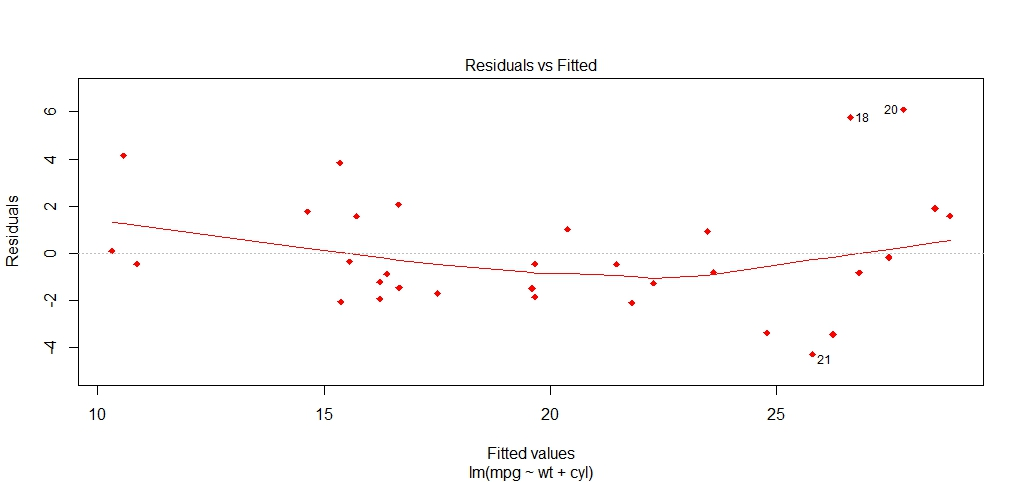
\includegraphics[width=0.95\linewidth]{./mtcarsDiagPlot1}
	
	\label{mtcarsDiagPlot1}
\end{figure}

\newpage
\subsubsection*{Plot 3 : Normal Probability Plot}
\begin{figure}[h!]
	\centering
	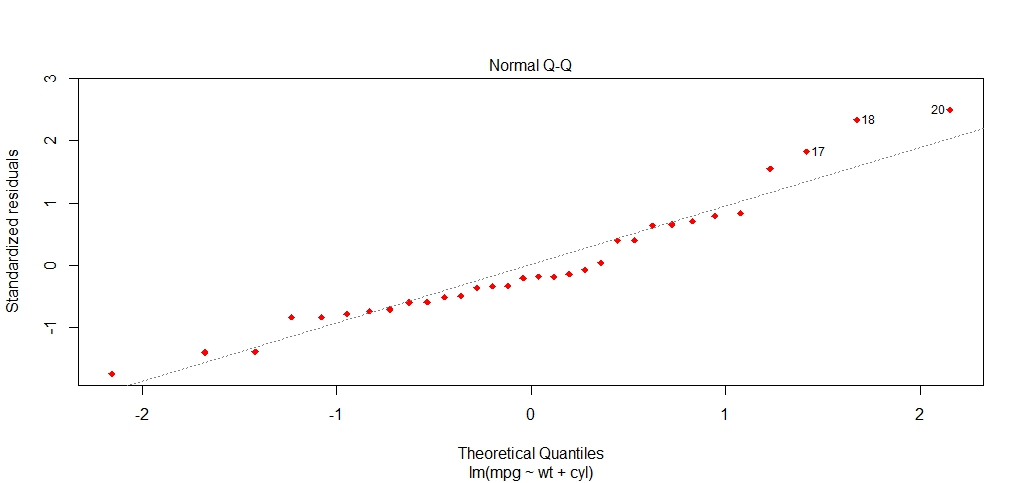
\includegraphics[width=0.95\linewidth]{./mtcarsDiagPlot2}
	
	\label{mtcarsDiagPlot2}
\end{figure}


This plot is used to assess the validity of the normality of the residuals.
\begin{figure}[h!]
	\centering
	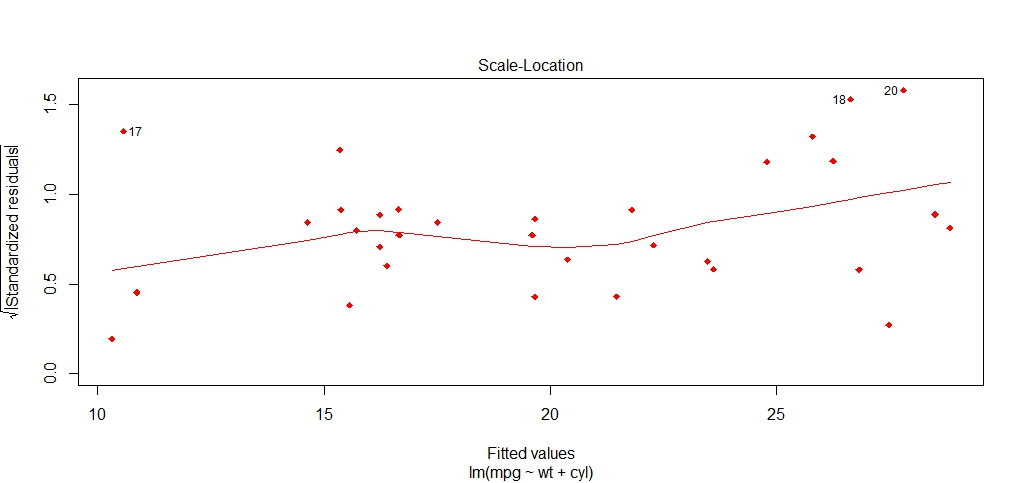
\includegraphics[width=0.95\linewidth]{./mtcarsDiagPlot3}
	
	\label{mtcarsDiagPlot3}
\end{figure}

\newpage
\subsubsection*{Plot 5 :  Cook's Distance}
\begin{figure}[h!]
	\centering
	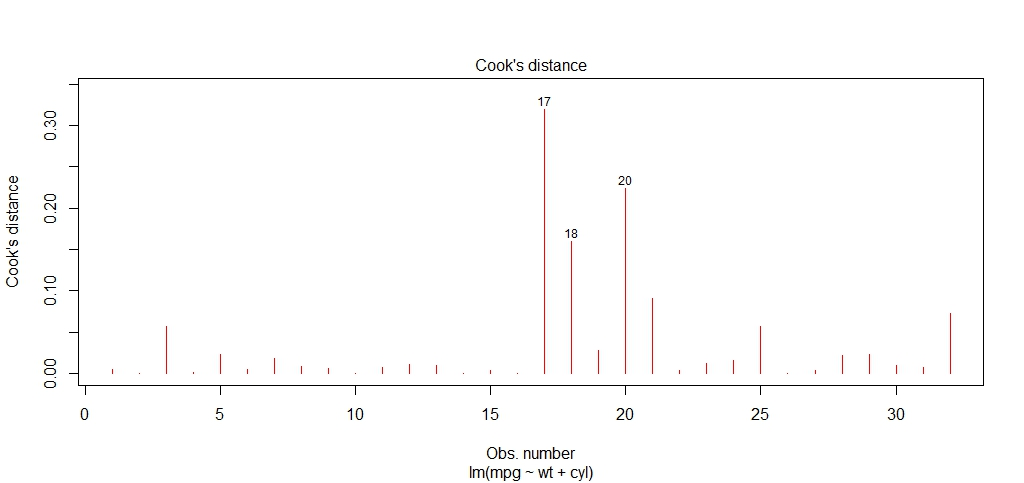
\includegraphics[width=0.95\linewidth]{./mtcarsDiagPlot4}
	
	\label{mtcarsDiagPlot4}
\end{figure}



\begin{figure}[h!]
	\centering
	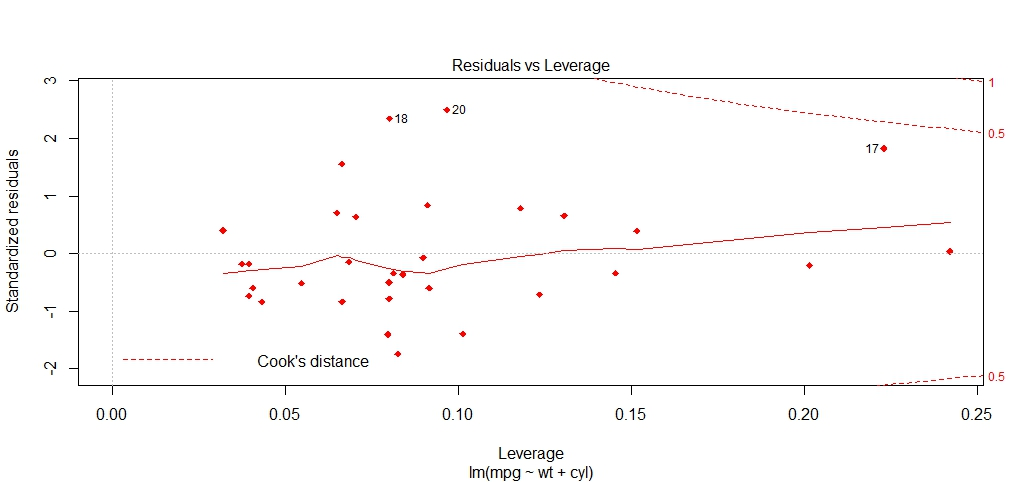
\includegraphics[width=0.9\linewidth]{./mtcarsDiagPlot5}
	
	\label{mtcarsDiagPlot5}
\end{figure}
\newpage

\subsubsection*{Plot 6 :  Cook's Distance vs Leverage}
\begin{figure}[h!]
	\centering
	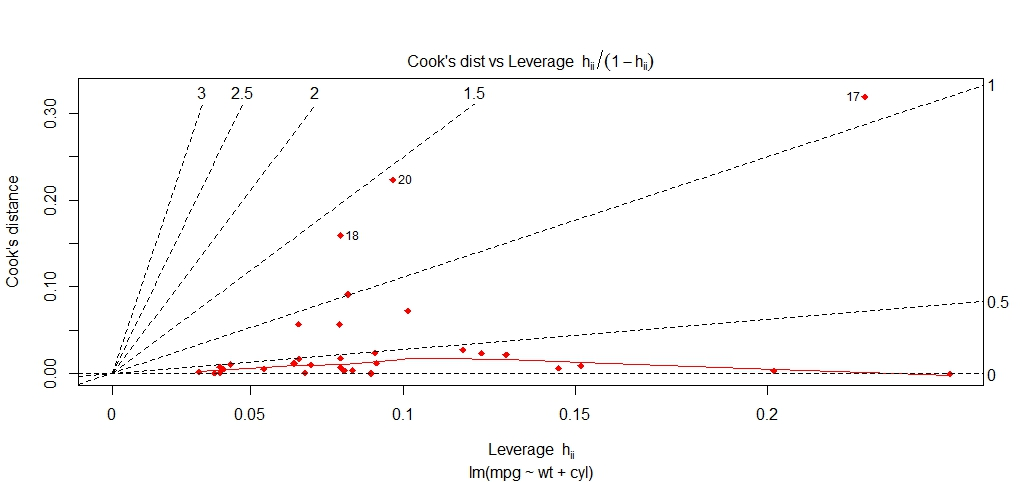
\includegraphics[width=0.95\linewidth]{./mtcarsDiagPlot6}
	
	\label{mtcarsDiagPlot6}
\end{figure}

Plot the four default plots together:
\begin{framed}
	\begin{verbatim}
	par(mfrow=c(4,1))
	plot(fittedmodel)
	par(opar)
	\end{verbatim}
\end{framed}

% http://www.columbia.edu/~cjd11/charles_dimaggio/DIRE/resources/R/rFunctionsList.pdf

\end{document}

